\documentclass[../searching.tex]{subfiles}
\begin{document}
% \paragraph{refers} 
% \url{https://tp-iiita.quora.com/The-Two-Pointer-Algorithm}


There are actually 50/900 problems on LeetCode are tagged as two pointers. Two pointer search algorithm are normally used to refer to searching that use two pointer in one for/while loop over the given data structure. Therefore, this part of algorithm gives linear performance as of $O(n)$. While, it does not refer to situation such as searching a pair of items in an array that sums up to a given target value, then two nested for loops are needed to search all the possible pairs. There are different ways to put these two pointers:
\begin{enumerate}
    \item Equi-directional:  Both start from the beginning: we have \textbf{slow-faster pointer}, \textbf{sliding window algorithm}.
    \item Opposite-directional: One at the start and the other at the end, they move close to each other and meet in the middle, (-> <-).
\end{enumerate}
In order to use two pointers, most times the data structure needs to be ordered in some way, and decrease the time complexity from $O(n^2)$ or $O(n^3)$ of two/three nested for/while loops to $O(n)$ of just one loop with two pointers and search each item just one time. In some cases, the time complexity is highly dependable on the data and the criteria we set. 

As shown in Fig.~\ref{fig:two pointer}, the pointer $i$ and $j$ can decide: a pair or a subarray (with all elements starts from i and end at j). We can either do search related with a pair or a subarray. For the case of subarray, the algorithm is called sliding window algorithm. As we can see, two pointers and sliding window algorithm can be used to solve K sum (Section~\ref{}), most of the subarray (Section~\ref{}), and string pattern match problems (Section~\ref{}). 
\begin{figure}[h!]
    \centering
    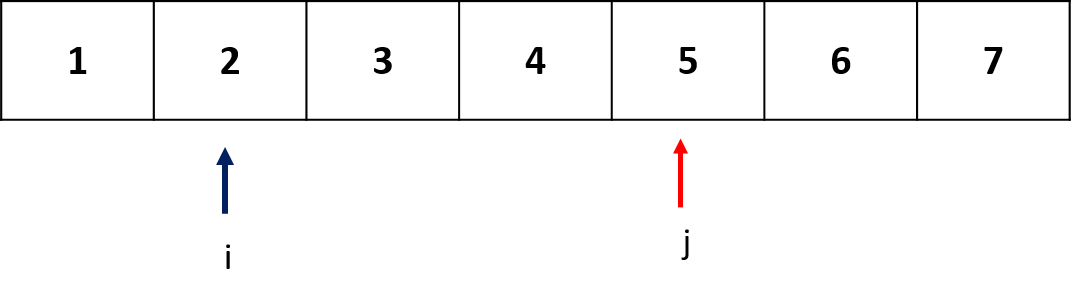
\includegraphics[width=0.9\columnwidth]{fig/two_pointers.png}
    \caption{Two pointer Example}
    \label{fig:two pointer}
\end{figure}

Two pointer algorithm is less of a talk and more of problem attached. We will explain this type of algorithm in virtue of both the leetcode problems and definition of algorihtms. 
% \subsection{Two Pointers Techniques}
To understand two pointers techniques, better to use examples, here we use two examples: use slow-faster pointer to find the median and Floyd's fast-slow pointer algorithm for loop detection in an array/linked list and two pointers to get two sum. 

\subsection{Slow-fast Pointer} 
\paragraph{Find middle node of linked list} The simpest example of slow-fast pointer application is to get the middle node of a given linked list. (LeetCode problem: 876. Middle of the Linked List)
\begin{lstlisting}[numbers=none]
Example 1 (odd length):

Input: [1,2,3,4,5]
Output: Node 3 from this list (Serialization: [3,4,5])

Example 2 (even length):

Input: [1,2,3,4,5,6]
Output: Node 4 from this list (Serialization: [4,5,6])
\end{lstlisting}
\begin{figure}[h]
    \centering
    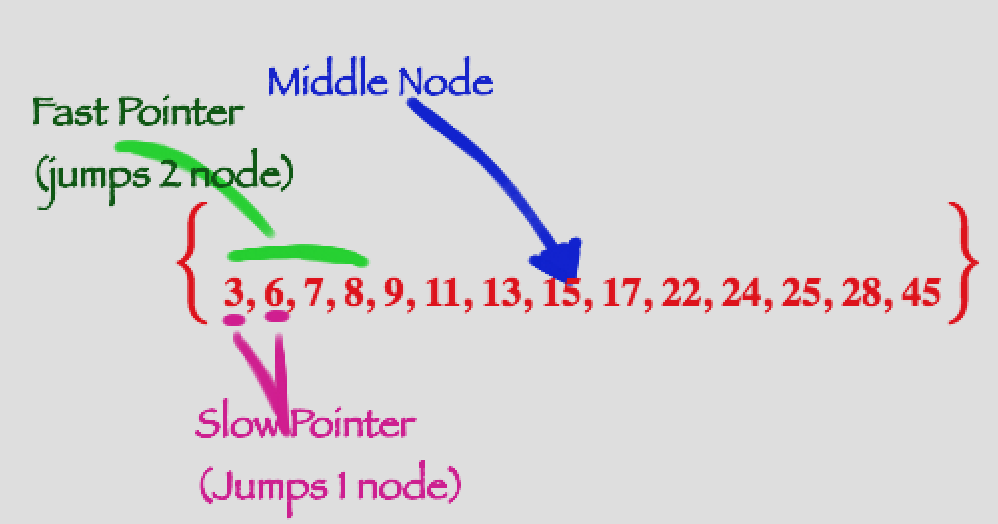
\includegraphics[width = 0.8\columnwidth]{fig/middle node of a given linked list.png}
    \caption{Slow-fast pointer to find middle}
    \label{fig:slow-faster}
\end{figure}
We place two pointers simultaneously at the head node, each one moves at different paces, the slow pointer moves one step and the fast moves two steps instead. When the fast pointer reached the end, the slow pointer will stop at the middle. For the loop, we only need to check on the faster pointer, make sure fast pointer and fast.next is not None, so that we can successfuly visit the fast.next.next. When the length is odd, fast pointer will point at the end node, because fast.next is None, when its even, fast pointer will point at None node, it terimates because fast is None. 
\begin{lstlisting}[language=Python]
def middleNode(self, head):
    slow, fast = head, head
    while fast and fast.next:        
        fast = fast.next.next
        slow = slow.next     
    return slow
\end{lstlisting}

\paragraph{Floyd's Cycle Detection (Floyd's Tortoise and Hare)} Given a linked list which has a cycle, as shown in Fig.~\ref{fig:floyd_cycle}. To check the existence of the cycle is quite simple. We do exactly the same as traveling by the slow and fast pointer above, each at one and two steps. (LeetCode Problem: 141. Linked List Cycle). The  code is pretty much the same with the only difference been that after we change the fast and slow pointer, we check if they are the same node. If true, a cycle is detected, else not. 
\begin{lstlisting}[language=Python]
def hasCycle(self, head):
    slow = fast = head
    while fast and fast.next:
        slow = slow.next
        fast = fast.next.next
        if slow == fast:
            return True
    return False
\end{lstlisting}

In order to know the starting node of the cycle. Here, we set the distance of the starting node of the cycle from the head is $x$, and $y$ is the distance from the start node to the slow and fast pointer's node, and $z$ is the remaining distance from the meeting point to the start node. 
\begin{figure}[h!]
    \centering
    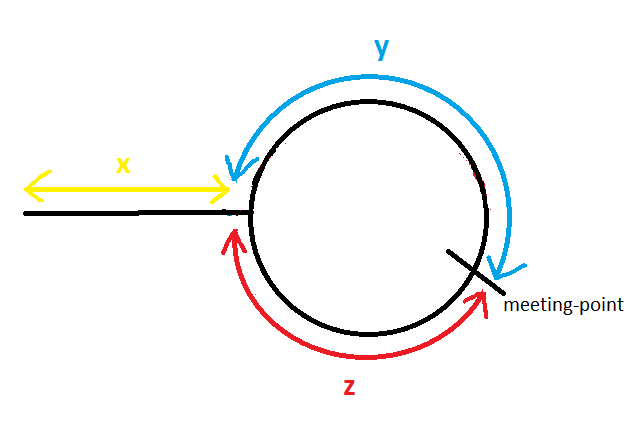
\includegraphics[width=0.7\columnwidth]{fig/TQoyH.png}
    \caption{Floyd's Cycle finding Algorithm}
    \label{fig:floyd_cycle}
\end{figure}

Now, let's try to device the algorithm. Both slow and fast pointer starts at position 0, the node index they travel each step is: [0,1,2,3,...,k] and [0,2,4,6,...,2k] for slow and fast pointer respectively. Therefore, the total distance traveled by the slow pointer is half of the distance travelled by the fat pointer. From the above figure, we have the distance travelled by slow pointer to be $d_s = x+y$, and for the fast pointer $d_f = x+y+z+y = x+2y+z$. With the relation $2*d_s = d_f$. We will eventually get $x = z$. Therefore, by moving slow pointer to the start of the linked list after the meeting point, and making both slow and fast pointer to move one node at a time, they will meet at the starting node of the cycle. (LeetCode problem: 142. Linked List Cycle II (medium)).
\begin{lstlisting}[language=Python]
def detectCycle(self, head):
    slow = fast = head
    bCycle = False
    while fast and fast.next:
        slow = slow.next
        fast = fast.next.next
        if slow == fast: # a cycle is found
            bCycle = True
            break
    
    if not bCycle:
        return None
    # reset the slow pointer to find the starting node       
    slow = head
    while fast and slow != fast:
        slow = slow.next
        fast = fast.next
    return slow
\end{lstlisting}
\begin{figure}[h!]
    \centering
    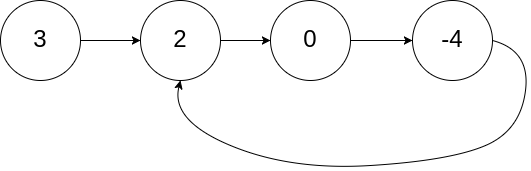
\includegraphics[width=0.6\columnwidth]{fig/circularlinkedlist.png}
    \caption{One example to remove cycle}
    \label{fig:cycle_remove}
\end{figure}
In order to remove the cycle as shown in Fig.~\ref{fig:cycle_remove}, the starting node is when slow and fast intersect, the last fast node before they meet. For the example, we need to set -4 node's next node to None. Therefore, we modify the above code to stop at the last fast node instead:
\begin{lstlisting}[language=Python]
    # reset the slow pointer to find the starting node       
    slow = head
    while fast and slow.next != fast.next:
        slow = slow.next
        fast = fast.next
    fast.next = None
\end{lstlisting}


\subsection{Opposite-directional Two pointer}
Two pointer is usually used for searching a pair in the array. There are cases the data is organized in a way that we can search all the result space by placing two pointers each at the start and rear of the array and move them to each other and eventually meet and terminate the search process. The search target should help us decide which pointer to move at that step.  This way, each item in the array is guaranteed to be visited at most one time by one of the two pointers, thus making the time complexity to be $O(n)$. Binary search used the technique of two pointers too, the left and right pointer together decides the current searching space, but it erase of half searching space at each step instead.

\paragraph{Two Sum - Input array is sorted} Given an array of integers that is already sorted in ascending order, find two numbers such that they add up to a specific target number. The function twoSum should return indices of the two numbers such that they add up to the target, where index1 must be less than index2.  (LeetCode problem: 167. Two Sum II - Input array is sorted (easy).)
\begin{lstlisting}[numbers=none]
Input: numbers = [2,7,11,15], target = 9
Output: [1,2]
Explanation: The sum of 2 and 7 is 9. Therefore index1 = 1, index2 = 2.
\end{lstlisting}

Due to the fact that the array is sorted which means in the array [s,s1 ..., e1, e], the sum of any two integer is in range of [s+s1, e1+e]. By placing two pointers each start from s and e, we started the search space from the middle of the possible range. [s+s1, s+e, e1+e].  Compare the target $t$ with the sum of the two pointers $v_1$ and $v_2$:
\begin{enumerate}
    \item  $t == v_1 + v_2$: found
    \item  $v_1+v_2 < t$: we need to move to the right side of the space, then we increase $v_1$ to get larger value.
    \item $v_1+v_2 > t$: we need to move to the left side of the space, then we decrease $v_2$ to get smaller value.
\end{enumerate}
\begin{lstlisting}[language=Python]
def twoSum(self, numbers, target):
    #use two pointers
    n = len(numbers)
    i, j  = 0, n-1
    while i < j:
        temp = numbers[i] + numbers[j]
        if temp == target:
            return [i+1, j+1]
        elif temp < target:
            i += 1
        else:
            j -= 1
    return []
\end{lstlisting}
% T1: If you see in the problem that you can do comparison and it is always one type of satisfactory element is in ahead of the other, this could be resolved by two pointers (slower and faster). Note: when the while loop stops, is there operations you need?

% Two pointers or three pointers are the most possible. \textit{Two pointers or three pointers is a superset of the sliding window algorithm, prefix sum too.} It can lower the complexity by one power level of n. 

%%%%%%%%%%%%%%%%%%%%%%Sliding Window Algorithm%%%%%%%%%%%%%%%%%%%%%%%%%%%%%%%%%%%%
\subsection{Sliding Window Algorithm}
\begin{figure}[h!]
    \centering
    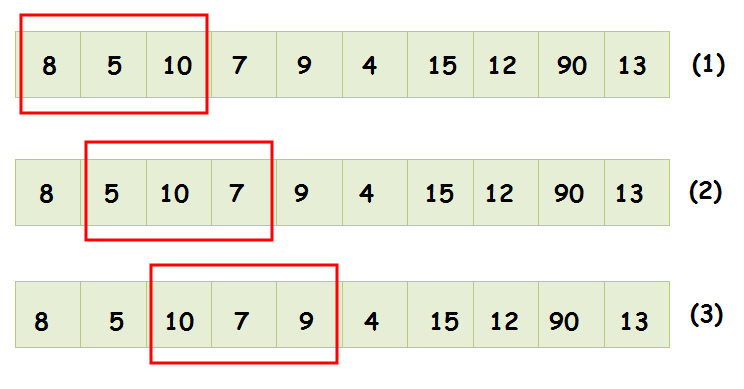
\includegraphics[width=0.7\columnwidth]{fig/sliding1.png}
    \caption{Sliding Window Algorithm}
    \label{fig:slide_window}
\end{figure}
Given an array, imagine that we have a fixed size window as shown in Fig.~\ref{fig:slide_window}, and we can slide it forward each time. If we are asked to compute the sum of each window, the bruteforce solution would be $O(kn)$ where k is the window size and n is the array size by using two nested for loops, one to set the starting point, and the other to compute the sum. A sliding window algorithm applied here used the property that the sum of the current window ($S_c$) can be computed from the last winodow ($S_l$) knowling the items that just slided out and moved in as $a_o$ and $a_i$. Then $S_c = S_l-a_o+a_i$. Not necessarily using sum, we generalize it as state, if we can compute $S_c$ from $S_l$, $a_o$ and $a_i$ in O(1), a function $S_c = f(S_l, a_o, a_i)$ then we name this \textbf{sliding window property}. Therefore the time complexity will be decreased to $O(n)$. 
\begin{lstlisting}[language=Python]
def fixedSlideWindow(A, k):
    n = len(A)
    if k >= n:
        return sum(A)
    # compute the first window
    acc = sum(A[:k])
    ans = acc
    # slide the window
    for i in range(n-k): # i is the start point of the window
        j = i + k # j is the end point of the window
        acc = acc - A[i] + A[j]
        ans = max(ans, acc)
    return ans
\end{lstlisting}

\paragraph{When to use sliding window} It is important to know when we can use sliding window algorithm, we summarize three important standards:
\begin{enumerate}
    \item It is a subarray/substring problem.
    \item \textbf{sliding window property:}T he requirement of the sliding window satisfy the sliding window property.
    \item \textbf{Completeness:} by moving the left and right pointer of the sliding window in a way that we can cover all the search space. Sliding window algorithm is about optimization problem, and by moving the left and right pointer we can search the whole searching space. \textbf{Therefore, to testify that if applying the sliding window can cover the whole search space and guarentee the completeness decide if the method works.}
\end{enumerate}

For example, 644. Maximum Average Subarray II (hard) does not satisfy the completeness. Because the average of subarray does not follow a certain order that we can decided how to move the window. 

\paragraph{Flexible Sliding Window Algorithm} Another form of sliding window where the window size is flexble, and it can be used to solve a lot of real problems related to subarray or substring that is conditioned on some pattern. Compared with the fixed size window, we can first fix the left pointer, and push the right pointer to enlarge the window in order to find a subarray satisfy a condition. Once the condition is met, we save the optimal result and shrink the window by moving the left pointer in a way that we can set up a new starting pointer to the window (shrink the window). At any point in time only one of these pointers move and the other one remains fixed.


\paragraph{Sliding Window Algorithm with Sum} In this part, we list two examples that we use flexible sliding window algorithms to solve subarray problem with sum condition. 

Given an array of n positive integers and a positive integer s, find the minimal length of a contiguous subarray of which the sum >= s. If there isn't one, return 0 instead. (LeetCode Problem: 209. Minimum Size Subarray Sum (medium)). 
\begin{lstlisting}[numbers=none]
Example: 

Input: s = 7, nums = [2,3,1,2,4,3]
Output: 2
Explanation: the subarray [4,3] has the minimal length under the problem constraint.
\end{lstlisting}
\begin{figure}[h!]
    \centering
    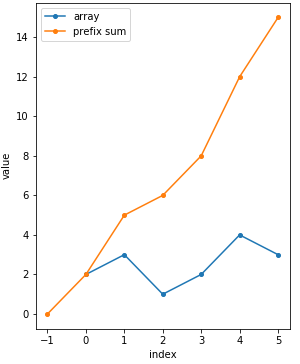
\includegraphics[width=0.5\columnwidth]{fig/prefixsum.png}
    \caption{The array and the prefix sum}
    \label{fig:prefix_sum_array}
\end{figure}
As we have shown in Fig.~\ref{fig:prefix_sum_array}, the prefix sum is the subarray starts with the first item in the array, we know that the sum of the subarray is monotonically increasing as the size of the subarray increase. Therefore, we place a 'window' with left and right as i and j at the first item first. The steps are as follows:
\begin{enumerate}
    \item Get the optimal subarray starts from current i, 0: Then we first move the j pointer to include enough items that sum[0:j+1]>=s, this is the process of getting the optimial subarray that starts with 0. And assume j stops at $e_0$
    \item Get the optimal subarray ends with current j, $e_0$: we shrink the window size by moving the i pointer forward so that we can get the optimal subarray that ends with current j and the optimal subarray starts from $s_0$. 
    \item Now, we find the optimal solution for subproblem [0:i,0:j](the start point in range [0, i] and end point in range [0,j]. Starts from next i and j, and repeat step 1 and 2.
\end{enumerate}

The above process is a standard flexible window size algorithm, and it is a complete search which searched all the possible result space. Both j and i pointer moves at most n, it makes the total operations to be at most 2n, which we get time complexity as $O(n)$. 
\begin{lstlisting}[language=Python]
def minSubArrayLen(self, s, nums):
    ans = float('inf')
    n = len(nums)
    i = j = 0
    acc = 0 # acc is the state
    while j < n:
        acc += nums[j]# increase the window size
        while acc >= s:# shrink the window to get the optimal result
            ans = min(ans, j-i+1)
            acc -= nums[i]
            i += 1
        j +=1
    return ans if ans != float('inf') else 0
\end{lstlisting}
\begin{bclogo}[couleur = blue!30, arrondi=0.1,logo=\bccrayon,ombre=true]{What happens if there exists negative number in the array? } Sliding window algorithm will not work any more, because the sum of the subarray is no longer monotonically increase as the size increase. Instead (1) we can use prefix sum and organize them in order, and use binary search to find all posible start index.  (2) use monotone stack (see  LeetCode probelm: 325. Maximum Size Subarray Sum Equals k, 325. Maximum Size Subarray Sum Equals k (hard)))
\end{bclogo}

More similar problems:
\begin{enumerate}
    \item 674. Longest Continuous Increasing Subsequence (easy)
\end{enumerate}

\paragraph{Sliding Window Algorithm with Substring} For substring problems, to be able to use sldiing window, s[i,j] should be gained from s[i,j-1] and s[i-1,j-1] should be gained from s[i,j-1]. Given a string, find the length of the longest substring without repeating characters. (LeetCode Problem: 3. Longest Substring Without Repeating Characters (medium))
\begin{lstlisting}[numbers=none]
Example 1:

Input: "abcabcbb"
Output: 3 
Explanation: The answer is "abc", with the length of 3. 

Example 2:

Input: "bbbbb"
Output: 1
Explanation: The answer is "b", with the length of 1.
\end{lstlisting}

First, we know it is a substring problem. Second, it askes to find substring that only has unique chars, we can use hashmap to record the chars in current window, and this satisfy the sliding window property. When the current window violates the condition ( a repeating char), we shrink the window in a way to get rid of this char in the current window by moving the i pointer one step after this char. 
\begin{lstlisting}[language=Python]
def lengthOfLongestSubstring(self, s):
    if not s:
        return 0
    n = len(s)
    state = set()
    i = j = 0
    ans = -float('inf')
    while j < n:
        if s[j] not in state:
            state.add(s[j])
            ans = max(ans, j-i)
        else:
            # shrink the window: get this char out of the window
            while s[i] != s[j]: # find the char
                state.remove(s[i])
                i += 1
            # skip this char
            i += 1
        j += 1
    return ans if ans != -float('inf') else 0
\end{lstlisting}

Now, let us see another example with string ang given a pattern to match. Given a string S and a string T, find the minimum window in S which will contain all the characters in T in complexity O(n). (LeetCode Problem: 76. Minimum Window Substring (hard))
\begin{lstlisting}[numbers=none]
Example:

Input: S = "ADOBECODEBANC", T = "ABC"
Output: "BANC"
\end{lstlisting}

In this problem, the desirable window is one that has all characters from T. The solution is pretty intuitive. We keep expanding the window by moving the right pointer. When the window has all the desired characters, we contract (if possible) and save the smallest window till now. The only difference compared with the above problem is the definition of desirable: we need to compare the state of current window with the required state in T. They can be handled as a hashmap with character as key and frequency of characters as value. 
\begin{lstlisting}[language=Python]
def minWindow(self, s, t):
    dict_t = Counter(t)
    state = Counter()
    required = len(dict_t)

    # left and right pointer
    i, j = 0, 0

    formed = 0
    ans = float("inf"), None # min len, and start pos

    while j < len(s):
        char = s[j]
        # record current state
        if char in dict_t:
            state[char] += 1
            if state[char] == dict_t[char]:
                formed += 1

        # Try and contract the window till the point where it ceases to be 'desirable'.
        # bPrint = False
        while i<=j and formed == required:
            # if not bPrint:
            #     print('found:', s[i:j+1], i, j)
            #     bPrint = True
            char = s[i]
            if j-i+1 < ans[0]:
                ans = j - i + 1, i
            # change the state
            if char in dict_t:
                state[char] -= 1
                if state[char] == dict_t[char]-1:
                    formed -= 1

            # Move the left pointer ahead,
            i += 1    
        
        # Keep expanding the window 
        j += 1  
        # if bPrint:
        #     print('move to:', s[i:j+1], i, j)
    return "" if ans[0] == float("inf") else s[ans[1] : ans[1] + ans[0]]
\end{lstlisting}

The process would be:
\begin{lstlisting}[numbers=none]
found: ADOBEC 0 5
move to: DOBECO 1 6
found: DOBECODEBA 1 10
move to: ODEBAN 6 11
found: ODEBANC 6 12
move to: ANC 10 13
\end{lstlisting}
\paragraph{Three Pointers and Sliding  Window Algorithm}
Sometimes, by manipulating two pointers are not enough for us to get the final solution. 
\begin{examples}
\item \textbf{930. Binary Subarrays With Sum.} In an array A of 0s and 1s, how many non-empty subarrays have sum S?
\begin{lstlisting}[numbers=none]
Example 1:

Input: A = [1,0,1,0,1], S = 2
Output: 4
Explanation: 
The 4 subarrays are bolded below:
[1,0,1,0,1]
[1,0,1,0,1]
[1,0,1,0,1]
[1,0,1,0,1]
\end{lstlisting}
\textit{Note: A.length <= 30000, 0 <= S <= A.length, A[i] is either 0 or 1.}

For example in the following problem, if we want to use two pointers to solve the problem, we would find we miss the case; like in the example $1, 0, 1, 0, 1$, when $j = 5$, $i = 1$, the sum is $2$, but the algorithm would miss the case of $i = 2$, which has the same sum value.
 
To solve this problem, we keep another index $i_hi$, in addition to the moving rule of $i$, it also moves if the sum is satisfied and that value is $0$. This is actually a Three pointer algorithm, it is also a mutant sliding window algorithm. 
\begin{lstlisting}[language=Python]
class Solution:
    def numSubarraysWithSum(self, A, S):
        i_lo, i_hi, j = 0, 0, 0 #i_lo <= j
        sum_window = 0
        ans = 0
        while j < len(A):

            sum_window += A[j]
                                     
            while i_lo < j and sum_window > S:
                sum_window -= A[i_lo]
                i_lo += 1
            # up till here, it is standard sliding window
            
            # now set the extra pointer at the same location of the i_lo
            i_hi = i_lo
            while i_hi < j and sum_window == S and not A[i_hi]:
                i_hi += 1
            if sum_window == S:
                ans += i_hi - i_lo + 1
                            
            j += 1 #increase the pointer at last so that we do not need to check if j<len again

        return ans
\end{lstlisting}
\end{examples}

\paragraph{Summary} Sliding Window is a powerful tool for solving certain subarray/substring related problems. The normal situations where we use sliding window is summarized:
\begin{itemize}
    \item Subarray: for an array with numerical value, it requires all positive/negative values so that the prefix sum/product has monotonicity. 
    \item Substring: for an array with char as value, it requires the state of each subarray does not related to the order of the characters (anagram-like state) so that we can have the sliding window property.
\end{itemize}

The steps of using sliding windows:
\begin{enumerate}
    \item Initialize the left and right pointer;
    \item Handle the right pointer and record the state of the current window;
    \item While the window is in the state of desirable: record the optimal solution, move the left pointer and record the state (change or stay unchanged).
    \item Up till here, the state is not desirable.  Move the right pointer in order to find a desirable window;
\end{enumerate}
\subsection{LeetCode Problems}
\paragraph{Sliding Window}
\begin{examples}
\item 76. Minimum Window Substring
\item 438. Find All Anagrams in a String
\item 30. Substring with Concatenation of All Words
\item 159. Longest Substring with At Most Two Distinct Characters
\item 567. Permutation in String
\item 340. Longest Substring with At Most K Distinct Characters
\item 424. Longest Repeating Character Replacement
\end{examples}
\end{document}